\documentclass[11pt]{amsart}

\usepackage[letterpaper,margin=1.15in]{geometry}
\usepackage[T1]{fontenc}
\usepackage{lmodern}
\usepackage{microtype}
\usepackage{amsmath,amssymb,amsthm,mathtools}
\usepackage{graphicx}
\graphicspath{{../figures/}}
\usepackage{booktabs}
\usepackage{enumitem}
\usepackage{needspace}
\usepackage{aliascnt}
\usepackage{xcolor}
\usepackage[colorlinks=true,linkcolor={blue!50!black},citecolor={blue!50!black},urlcolor={blue!50!black}]{hyperref}
\usepackage[capitalize,nameinlink]{cleveref}
\hypersetup{pdftitle={An upper bound for the Euclidean travelling salesman constant},pdfauthor={Devin O'Keefe}}
\raggedbottom
\makeatletter
% With \raggedbottom every page has zero badness, so any negative penalty attracts the page break.
% The default \@secpenalty (-300) and the \penalty-100 inside \needspace both end pages early;
% this \needspace breaks only when less than #1 remains on the page.
\@secpenalty=0
\renewcommand{\needspace}[1]{\par\begingroup\setlength{\dimen@}{#1}%
  \dimen@ii\pagegoal \advance\dimen@ii-\pagetotal
  \ifdim\dimen@>\dimen@ii \ifdim\dimen@ii>\z@\vfil\fi\penalty-\@M\fi\endgroup}
\makeatother
\renewcommand{\topfraction}{0.85}
\renewcommand{\bottomfraction}{0.6}
\renewcommand{\textfraction}{0.1}
\renewcommand{\floatpagefraction}{0.75}

% ------------------------------------------------------------------ paragraphs
% Half a line of space between paragraphs, and no indent.  Theorems, proofs and the run-in headings
% defined below are set off by a full line.
\setlength{\parskip}{0.5\baselineskip plus 1pt}
\setlength{\parindent}{0pt}
\makeatletter
% The class takes \parskip off the space above a theorem, and \parskip follows the space below it.
\def\thm@space@setup{%
  \thm@preskip=1\baselineskip \@plus.2\baselineskip \@minus.2\baselineskip
  \thm@postskip=.5\baselineskip \@plus.2\baselineskip \@minus.2\baselineskip}
\makeatother

% ------------------------------------------------------------------ theorem environments
% Propositions, lemmas and remarks share the counter of theorems.  Each gets an alias
% counter, so that \cref names the environment correctly with every version of cleveref.
\newtheorem{thm}{Theorem}[section]
\newaliascnt{prop}{thm}
\newtheorem{prop}[prop]{Proposition}
\aliascntresetthe{prop}
\newaliascnt{lem}{thm}
\newtheorem{lem}[lem]{Lemma}
\aliascntresetthe{lem}
\theoremstyle{definition}
\newaliascnt{rem}{thm}
\newtheorem{rem}[rem]{Remark}
\aliascntresetthe{rem}
\numberwithin{equation}{section}
\numberwithin{figure}{section}
\numberwithin{table}{section}
\crefname{thm}{Theorem}{Theorems}
\crefname{prop}{Proposition}{Propositions}
\crefname{lem}{Lemma}{Lemmas}
\crefname{rem}{Remark}{Remarks}
\crefname{figure}{Figure}{Figures}

% ------------------------------------------------------------------ notation
\newcommand{\R}{\mathbb{R}}
\newcommand{\Z}{\mathbb{Z}}
\newcommand{\E}{\mathbb{E}}
\newcommand{\eps}{\varepsilon}
\renewcommand{\Pr}{\mathbb{P}}

% ------------------------------------------------------------------ run-in headings
% The steps of Section 4 and the topics of Sections 5.2 and 5.3: an italic heading that opens a
% paragraph, with half a line of space above it in addition to the space between paragraphs.
\newcommand{\runin}[1]{\par\medskip\emph{#1}}

% ------------------------------------------------------------------ results of the computation
% Written by tools/paper_numbers.py from the records in runs/; do not edit.
\newcommand{\LeanMaxK}{9}
\newcommand{\BoundFiveUp}{0.8789}
\newcommand{\CellsFive}{4.8\cdot10^{7}}
\newcommand{\ResultCountWord}{five}
\newcommand{\MainK}{9}
\newcommand{\MainPoints}{ten}
\newcommand{\MainH}{11/5}
\newcommand{\MainBound}{0.8618}
\newcommand{\MainBoundShort}{0.861716}
\newcommand{\MainTotal}{4{,}430{,}997{,}795{,}015{,}293{,}889}
\newcommand{\MainCells}{1.6\cdot10^{13}}
\newcommand{\MainCellsFormula}{4^{9}\cdot6^{10}}
\newcommand{\MainCellsRemark}{, about as many as that grid, though a cell takes more work for larger $k$}
\newcommand{\MainGapTuples}{262{,}144}
\newcommand{\MainTableEntries}{4284}
\newcommand{\MainProofFraction}{5\,\mathsf{A}_0/(6^{10}\cdot2^{32}\cdot9\cdot11)}
\newcommand{\MainMargin}{8\cdot10^{-5}}
\newcommand{\LossFive}{0.0046}
\newcommand{\SimBlocks}{4\cdot10^{8}}
\newcommand{\IntegralMarginMin}{4.8\cdot10^{-8}}
\newcommand{\IntegralMarginMax}{1.9\cdot10^{-4}}
\newcommand{\SimCostMain}{0.861722\pm0.000008}
\newcommand{\BracketFullK}{7}
\newcommand{\LossMain}{0.0077}
\newcommand{\MainLimit}{0.854}
\newcommand{\DongCaoSamples}{4\cdot10^{6}}
\newcommand{\DongCaoRule}{0.87467\pm0.00012}
\newcommand{\DongCaoGap}{0.000493\pm0.000001}
\newcommand{\LimitSamples}{4\cdot10^{7}}
\newcommand{\LimitError}{0.00004}
\newcommand{\LimitStepFirst}{0.007}
\newcommand{\LimitStepLast}{0.003}


% abstract set as in the article class: centred bold heading above an indented block
\makeatletter
\renewenvironment{abstract}{%
  \global\setbox\abstractbox=\vtop \bgroup
    \normalfont\Small
    \list{}{\labelwidth\z@ \leftmargin3pc \rightmargin\leftmargin
      \listparindent\normalparindent \itemindent\z@ \parsep\z@ \@plus\p@
      \let\fullwidthdisplay\relax}%
    \item\relax{\centering\bfseries\abstractname\par}\vskip0.5\baselineskip
    \ignorespaces
}{%
  \endlist\egroup
  \ifx\@setabstract\relax \@setabstracta \fi
}
\makeatother

\begin{document}

\title[An upper bound for the travelling salesman constant]{An upper bound for the Euclidean\\ travelling salesman constant}

\author{Devin O'Keefe}
\address{Independent Researcher}
\email{okeefede@tcd.ie}

\subjclass[2020]{Primary 60D05; Secondary 90C27, 68V05}
\keywords{travelling salesman problem, Beardwood--Halton--Hammersley theorem, computer-assisted proof, integer arithmetic}

\begin{abstract}
By a theorem of Beardwood, Halton and Hammersley, the length of a shortest tour through $n$ independent uniform random points in the unit square is asymptotic to $\beta\sqrt n$ for a constant $\beta$, which numerical estimates place near $0.712$. We prove $\beta<\MainBound$. The best earlier upper bound, $\beta\le0.8810$, is in a recent preprint of Dong and Cao. They cut the square into strips, take the points of each strip in blocks of six, and choose the order of visits within a block by a rule that is constant on the cells of a finite partition of the space of blocks. In each cell they bound the expected length of each segment of the path by the square root of its second moment. We change this last step: the length of a segment is a convex function of the positions of the points, and we bound its expectation by the Edmundson--Madansky inequality, a standard bound for convex functions, on a mesh much finer than the partition. For blocks of six points, $\CellsFive$ cells then give a better bound than their $1.6\cdot10^{13}$ cells. This makes blocks of \MainPoints{} points feasible, and these give the bound $\MainBound$. The proof ends in a computation in integer arithmetic, which three programs in different languages carry out with identical results.

\end{abstract}

\maketitle

\section{Introduction}\label{sec:intro}

\subsection{The constant}

Let $X_1,X_2,\dots$ be independent random points, uniformly distributed in the unit square, and let $L_n$ be the length of a shortest closed tour through $X_1,\dots,X_n$. Beardwood, Halton and Hammersley \cite{BeardwoodHaltonHammersley1959} proved that there is a constant $\beta$ such that
\[
\lim_{n\to\infty}\frac{L_n}{\sqrt n}=\beta\qquad\text{almost surely.}
\]
The value of $\beta$ is not known. Numerical estimates are $0.7124\pm0.0002$ \cite{JohnsonMcGeochRothberg1996} and $0.7120\pm0.0002$ \cite{PercusMartin1996}. The proved lower and upper bounds leave a much wider interval (\cref{tab:history}). The constant is number~12 in the online list of optimisation constants \cite{optimisation-constants-repo}.

All upper bounds for $\beta$ so far come from the strip construction of \cite{BeardwoodHaltonHammersley1959}: cut the square into horizontal strips of height $h/\sqrt n$ and visit the points of each strip in the order of their first coordinates, one strip after another. With $h=\sqrt3$ this gives $\beta\le0.92116\ldots$\,. Few \cite{Few1955} had used a very similar argument for arbitrary points, as Steinerberger notes \cite[Section~2.2]{Steinerberger2015}.\footnote{Sections, tables and remarks of \cite{Steinerberger2015} and \cite{GaudioGuan2026} are cited by their numbers in the arXiv versions; for the article \cite{CarlssonYu2026} we cite its preprint \cite{YuCarlsson2023}, with the numbers of the preprint.} Exchanging two consecutive points of a strip in certain configurations improves the bound by a small amount \cite{Steinerberger2015}. The same paper proposes to optimise the order of visits within groups of consecutive points; for disjoint groups of six points, with the first and the last point of each group kept in place, a simulation gave about $0.8902$ \cite[Section~2.5]{Steinerberger2015}.

Yu and Carlsson \cite{YuCarlsson2023} were the first to turn this proposal into a proved bound. Take the points of a strip in blocks of $k+1$ consecutive points, each block sharing its last point with the next, and visit the $k-1$ interior points of each block in the best order. This gives
\begin{equation}\label{eq:tuple}
\beta\le\frac{1}{kh}\,\E\min_\pi L_\pi ,
\end{equation}
where $L_\pi$ is the length of the path that visits the interior points of a random block in the order $\pi$, measured after a magnification by the factor $h$ (hence the $h$ in the denominator); precise definitions are in \cref{sec:blocks}.

The right-hand side is an integral over $2k+1$ variables of a minimum of $(k-1)!$ functions, and the difficulty is to bound it rigorously. For $k=4$ this is done in \cite{YuCarlsson2023}, with a partition of the domain found by a decision tree, one order for each part, and interval arithmetic; the published article \cite{CarlssonYu2026} gives $\beta<0.9038$.\footnote{The preprint \cite{YuCarlsson2023} stated $0.90304$, which is also the value in the list \cite{optimisation-constants-repo} at the time of writing; \cref{tab:history} follows the published articles, and the value of the article is quoted from its abstract.} Gaudio and Guan \cite{GaudioGuan2026} improved the bound to $0.90367$ by allowing a point near the boundary of a strip to be visited from the adjacent strip. They also estimated the right-hand side of \eqref{eq:tuple} by simulation: for $h=\sqrt{3.75}\approx1.94$ it is about $0.8748$ for $k=5$, $0.8650$ for $k=7$ and $0.8622$ for $k=8$ \cite[Table~2]{GaudioGuan2026}.

The best bound so far, $\beta\le0.8810$, was proved with $k=5$ and $h=2$ by Dong and Cao in a preprint of 2~October 2026 \cite{DongCao2026}. They show first that, for blocks of six points, every rule that chooses the order of visits from the positions of the points gives an upper bound for $\beta$ \cite[Theorem~4]{DongCao2026}. The space of blocks is then divided into the cells of a product grid, with one order for each cell, and in each cell the expected length of a segment is bounded by the square root of its second moment.

They also give a statistical estimate: a bound computed from a random sample, which holds with probability at least $1-10^{-4}$ and is $0.8749$ for their sample \cite[Section~4.3]{DongCao2026}; it is not a proved bound, and \cref{tab:history} does not list it. Their conclusion names finer partitions and larger blocks as sources of further improvement.

\begin{table}[ht]
\centering
\caption{Proved bounds for the constant $\beta$. The upper bound of \cite{BeardwoodHaltonHammersley1959} is given as corrected in \cite{Steinerberger2015}; the value $0.92037$ printed in \cite{BeardwoodHaltonHammersley1959} is a numerical error. The lower bound of \cite{Steinerberger2015} is given as corrected in \cite{GaudioJaillet2020}, to $5/8+19/10368$. The last column gives the number $k$ of \eqref{eq:tuple} for the bounds that come from blocks.}
\label{tab:history}
\begin{tabular}{@{}llll@{}}
\toprule
 & Bound & Source & $k$ \\
\midrule
Lower & $0.625$ & Beardwood, Halton, Hammersley \cite{BeardwoodHaltonHammersley1959} & \\
      & $0.6268$ & Steinerberger \cite{Steinerberger2015} & \\
      & $0.6277$ & Gaudio, Jaillet \cite{GaudioJaillet2020} & \\
      & $0.6421$ & Dong, Cao \cite{DongCao2026}, preprint & \\
\midrule
Upper & $0.92116\ldots$ & Beardwood, Halton, Hammersley \cite{BeardwoodHaltonHammersley1959} & $1$ \\
      & $0.92116\ldots-\tfrac{9}{16}\cdot10^{-6}$ & Steinerberger \cite{Steinerberger2015} & \\
      & $0.9038$ & Carlsson, Yu \cite{CarlssonYu2026} & $4$ \\
      & $0.90367$ & Gaudio, Guan \cite{GaudioGuan2026} & $4$ \\
      & $0.8810$ & Dong, Cao \cite{DongCao2026}, preprint & $5$ \\
      & $\MainBound$ & \cref{thm:main} & $\MainK$ \\
\bottomrule
\end{tabular}
\end{table}

\subsection{The result}

\begin{thm}\label{thm:main}
The constant $\beta$ of Beardwood, Halton and Hammersley satisfies $\beta<\MainBound$.
\end{thm}

The proof uses blocks of \MainPoints{} points ($k=\MainK$) and strips with $h=\MainH$. With smaller blocks the same method gives weaker bounds, starting from $\beta<\BoundFiveUp$ for $k=5$ and $h=2$ (\cref{thm:computation}).

\subsection{The method}

We take two things from \cite{DongCao2026}: rules that are constant on the cells of a product grid, and the theorem that every rule gives an upper bound for $\beta$. Since that preprint is recent and treats $k=5$, we prove the theorem in full for general $k$ (\cref{thm:block}). What we change is how the expected length of a segment between two points of a block is bounded in a cell.

The square root of the second moment exceeds the expected length by an amount that depends on how much the length varies within the cell, so a good bound needs small cells. The bound $0.8810$ was obtained with a grid of $12^5\cdot20^6\approx1.6\cdot10^{13}$ cells, reduced by symmetry \cite{DongCao2026}.

We use instead the fact that the length of a segment is a convex function of the gaps of the block (the horizontal distances between consecutive points) and of the heights of its points. On an interval, the expectation of a convex function is at most the expectation of its chord; this is the Edmundson--Madansky inequality \cite{Edmundson1957,Madansky1959}. We apply it to one variable at a time, on a mesh much finer than the cells (\cref{prop:segment}). A cell confines each gap and each height to an interval; where the interval of a gap is unbounded, we first truncate the gap and add the expectation of the excess (\cref{lem:unbounded}).

The accuracy of the bound for a segment is then set by the mesh and by the level of the truncation, which can be changed without changing the cells. The cells matter only because the rule chooses the same order throughout a cell. As with the second-moment bound of \cite{DongCao2026}, our bound for a segment depends on the cell only through a few integers (\cref{sec:segment}), so that for $k=\MainK$ all of its values fit in a table with \MainTableEntries{} entries.

With $4^5\cdot6^6\approx\CellsFive$ cells we obtain $\BoundFiveUp$ for $k=5$ and $h=2$, against $0.8810$ from the grid of $1.6\cdot10^{13}$ cells. This leaves room for larger blocks. The computation for $k=\MainK$ has $\MainCellsFormula\approx\MainCells$ cells\MainCellsRemark.

The proof of \cref{thm:main} ends in a finite computation. Every quantity in it is rounded to an integer at a fixed scale, in the direction that makes the bound larger, so that only integer arithmetic is used (\cref{sec:integers}). We carried out the computation with three programs, in Python, C and Rust, which share no code and agree on every entry of the table of bounds for the segments, on all $\MainGapTuples$ cell sums of \cref{sec:recipe} and on the total (\cref{sec:computation}).

% \looseness keeps this paragraph at five lines, so that the pages break where they did.
\looseness=1 The total for $k=\MainK$ was also confirmed in the proof assistant Lean, by an evaluation in compiled code that the Lean kernel does not check. The agreement of these computations is evidence against errors of implementation, not against an error in the proofs, and the proofs of \cref{sec:blocks,sec:cells,sec:integers} are not formalised. \Cref{sec:programs} says what these checks can and cannot show.

The separate steps of the method are not new. Applying the Edmundson--Madansky inequality to one independent variable at a time, on each interval of a partition, is a standard way to bound the expectation of a convex function in stochastic programming \cite{KallWallace1994,HuangZiembaBenTal1977}, and one integral is bounded from above with chords in \cite[Remark~6]{YuCarlsson2023}. A program that Carlsson published in 2024 as a complement to \cite{CarlssonYu2026,YuCarlsson2023} already uses convexity on a grid: it bounds the length of the path of an order on a cell by the largest of its values at the corners of the cell, and is designed to take for each cell the order for which this bound is smallest.\footnote{\url{https://github.com/johngcarlsson-usc/tsp-constant-discretization}, accessed 9~October 2026.} Rigorous arithmetic has been used before (intervals in \cite{YuCarlsson2023}, rational numbers in \cite{DongCao2026}), and two of the three identities by which our programs shorten the sum over the cells are used in \cite{DongCao2026} (\cref{sec:programs}). We add the combination of these steps and the scheme of integer arithmetic of \cref{sec:integers}.

The bound is still far from the numerical estimates near $0.712$. For given $k$ and $h$ no rule gives less than the right-hand side of \eqref{eq:tuple}, which for $k=\MainK$ and $h=\MainH$ is about $\MainLimit$ by simulation (\cref{tab:controls}), and in the simulations of \cref{sec:remarks} the gain from each further point in a block is small.

\section{The block bound}\label{sec:blocks}

We prove that every rule for choosing the order of visits within a block gives an upper bound for $\beta$ (\cref{thm:block}).

\subsection{The constant in terms of a Poisson process}

For a finite set $A\subset\R^2$ let $L(A)$ be the length of a shortest closed tour through the points of $A$, with $L(A)=0$ if $A$ has fewer than two points. In this notation the $L_n$ of \cref{sec:intro} is $L(\{X_1,\dots,X_n\})$. We use the following standard consequence of the theorem of Beardwood, Halton and Hammersley \cite{BeardwoodHaltonHammersley1959,Steele1997}. It is stated in this form in \cite[equation~(5)]{DongCao2026}; the short proof follows the sketch in \cite[Section~2.1]{Steinerberger2015}, attributed there to Steele.

\begin{lem}\label{lem:poisson}
Let $\Pi$ be a Poisson process of intensity $1$ in the plane, and let $\Lambda_W=[0,W]^2$. Then
\[
\lim_{W\to\infty}\frac{\E\,L(\Pi\cap \Lambda_W)}{W^2}=\beta .
\]
\end{lem}

\begin{proof}
Put $\ell_n=\E\,L_n$. By a theorem of Few \cite{Few1955}, any $n\ge1$ points of the unit square lie on a path of length at most $\sqrt{2n}+1.75$. Closing the path adds at most $\sqrt2$, so $L(A)\le c\sqrt n$ with $c=2\sqrt2+1.75$ for every set $A$ of $n\ge1$ points in the unit square, and $\ell_n/\sqrt n\to\beta$ by bounded convergence. Hence for every $\eps>0$ there is a constant $C_\eps$ with $|\ell_n-\beta\sqrt n|\le\eps\sqrt n+C_\eps$ for all $n\ge0$.

Let $N$ be the number of points of $\Pi$ in $\Lambda_W$. It has the Poisson distribution with mean $W^2$, and given $N=n$ the points are independent and uniform in $\Lambda_W$. Scaling by $W$ gives $\E\,L(\Pi\cap \Lambda_W)=W\,\E\,\ell_N$, and therefore
\[
\bigl|\E\,L(\Pi\cap \Lambda_W)-\beta W\,\E\sqrt N\bigr|\le \eps W\,\E\sqrt N+C_\eps W .
\]
By Jensen's inequality, $\E\sqrt N\le W$. In the other direction, $\sqrt N-W=(N-W^2)/(\sqrt N+W)\ge-|N-W^2|/W$ and $\E|N-W^2|\le(\operatorname{Var}N)^{1/2}=W$, so $\E\sqrt N\ge W-1$. Dividing by $W^2$ and letting $W\to\infty$ and then $\eps\to0$ gives the claim.
\end{proof}

\subsection{Blocks, orders and rules}

Fix an integer $k\ge1$ and a real number $h>0$. Let $Z_1,\dots,Z_k$ be exponential random variables with mean $1$ and let $U_0,\dots,U_k$ be uniform on $[0,1]$, all independent. Put
\[
P_i=\bigl(Z_1+\dots+Z_i,\;h^2U_i\bigr),\qquad 0\le i\le k .
\]
We call $(P_0,\dots,P_k)$ a \emph{block}, the $Z_i$ its \emph{gaps} and the $U_i$ its \emph{heights}; the height of a point is its second coordinate divided by $h^2$. A block is a copy, magnified by the factor $h$, of $k+1$ consecutive points of a Poisson process of intensity $1$ in a horizontal strip of height $h$: there the horizontal distances between consecutive points are exponential with mean $1/h$ and the vertical coordinates are uniform on an interval of length $h$. The proof of \cref{thm:block} makes this precise.

An \emph{order} is a permutation $\pi$ of $\{1,\dots,k-1\}$. It stands for the path that starts at $P_0$, visits the \emph{interior points} $P_1,\dots,P_{k-1}$ in the order $P_{\pi(1)},\dots,P_{\pi(k-1)}$, and ends at $P_k$; we write $L_\pi$ for the length of this path. A \emph{rule} is a measurable map $\rho$ from $[0,\infty)^k\times[0,1]^{k+1}$ to the set of orders. It chooses an order from the gaps and heights of the block, and we write $L_\rho$ for the length of the path it chooses (\cref{fig:strip}).

\begin{figure}[ht]
\centering
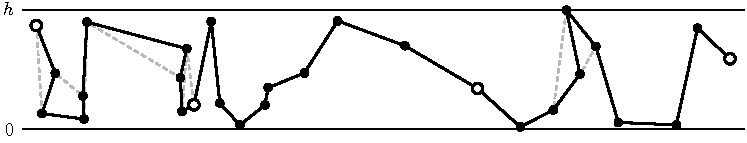
\includegraphics[width=\textwidth]{fig_strip}
\caption{Three consecutive blocks of a strip for $k=\MainK$ and $h=\MainH$, drawn from a simulation. Open circles mark the first and the last point of each block. The solid line is the path chosen by the rule of \cref{sec:computation} for \cref{thm:main}; where it differs from the order of the first coordinates, that order is shown by a dashed line.}
\label{fig:strip}
\end{figure}

\begin{thm}[Block bound]\label{thm:block}
For every integer $k\ge1$, every $h>0$ and every rule $\rho$,
\[
\beta\le\frac{\E\,L_\rho}{kh}.
\]
\end{thm}

We call $\E\,L_\rho/(kh)$ the \emph{value} of the rule $\rho$. For $k=1$ there is one order, and the value is the expected distance between consecutive points of a strip; this is the bound of \cite{BeardwoodHaltonHammersley1959}, where $h=\sqrt3$. For the rule that chooses a shortest path (the first one in a fixed list of the orders, if there are several), the theorem is the bound \eqref{eq:tuple} stated in \cite[Section~3.1]{YuCarlsson2023}; we call the value of this rule the \emph{shortest-path value} for $k$ and $h$, and no rule has a smaller value.

The computation of \cite{YuCarlsson2023} already uses a rule of another kind, which chooses one order on each part of a partition; this order need not be shortest at every point of the part. For arbitrary rules and $k=5$ the theorem is Theorem~4 of \cite{DongCao2026}, and the proof below follows the proof given there, with $5$ replaced by $k$ and the strips joined in a slightly different way.

\begin{proof}
Every path in a block has length at most $k(Z_1+\dots+Z_k+h^2)$, so $\E\,L_\rho<\infty$.

Let $\Pi$ be a Poisson process of intensity $1$ in the plane, let $q\ge1$ be an integer and $W=qh$. For $1\le j\le q$ let $S_j=[0,\infty)\times[(j-1)h,jh)$. Almost surely no point of $\Pi$ has second coordinate $W$, and the points of $\Pi$ in $S_j$ have distinct first coordinates; let $P^j_1,P^j_2,\dots$ be these points in increasing order of the first coordinate. Add an auxiliary point $P^j_0$ with first coordinate $0$ and second coordinate $(j-1)h+Y^j_0$, where $Y^j_0$ is uniform on $[0,h)$ and independent of everything else. For $i\ge1$ let $\Delta^j_i$ be the first coordinate of $P^j_i$ minus that of $P^j_{i-1}$, and let $(j-1)h+Y^j_i$ be the second coordinate of $P^j_i$. Then the $\Delta^j_i$, $i\ge1$, are independent and exponential with mean $1/h$, the $Y^j_i$, $i\ge0$, are independent and uniform on $[0,h)$, and the two families are independent of each other: the first coordinates of the points in $S_j$ form a Poisson process of intensity $h$ on $[0,\infty)$, and the second coordinates are independent marks \cite{Kingman1993}.

For $b\ge0$, the points $P^j_{kb},P^j_{kb+1},\dots,P^j_{k(b+1)}$ form the $b$th block of the strip. Translating them so that $P^j_{kb}$ has first coordinate $0$ and the lower edge of the strip has second coordinate $0$, and then multiplying by $h$, gives $k+1$ points with the distribution of a block: the gaps are $h\Delta^j_{kb+1},\dots,h\Delta^j_{kb+k}$ and the heights are $Y^j_{kb}/h,\dots,Y^j_{kb+k}/h$. Let the rule $\rho$ choose an order for it, and let $C^j_b$ be the length of the corresponding path from $P^j_{kb}$ to $P^j_{k(b+1)}$ in the strip. Then $C^j_b$ has the distribution of $L_\rho/h$.

Let $K_j$ be the number of points of $\Pi$ in $S_j\cap \Lambda_W$ and $B_j=1+\lfloor K_j/k\rfloor$. The paths of the blocks $0,1,\dots,B_j-1$ share endpoints and join to a walk $\Gamma_j$ from $P^j_0$ to $P^j_{kB_j}$, whose length we denote by $|\Gamma_j|$. Since $kB_j>K_j$, this walk visits every point of $\Pi$ in $S_j\cap \Lambda_W$.

The $b$th block is used, that is $b<B_j$, exactly when $kb\le K_j$. For $b=0$ this always holds. For $b\ge1$ it is the event $\Delta^j_1+\dots+\Delta^j_{kb}\le W$, which is determined by $\Delta^j_1,\dots,\Delta^j_{kb}$. The length $C^j_b$ is a function of $\Delta^j_{kb+1},\dots,\Delta^j_{kb+k}$ and $Y^j_{kb},\dots,Y^j_{kb+k}$, so it is independent of this event; this is the argument of Wald's identity. (The last block that is used contains the gap across the line $x=W$, which tends to be longer than a typical gap. This does not matter: each term of the sum below belongs to a fixed $b$, and none is conditioned on $b$ being the last index used. Nor need the lengths $C^j_b$ for different $b$ be independent; they are not, since consecutive blocks share a point.) Since all terms are non-negative,
\begin{equation}\label{eq:strip}
\E\,|\Gamma_j|=\sum_{b\ge0}\E\bigl[C^j_b\,;\,b<B_j\bigr]=\sum_{b\ge0}\Pr(b<B_j)\,\E\,C^j_b=\E B_j\cdot\frac{\E\,L_\rho}{h}\le\Bigl(1+\frac{hW}{k}\Bigr)\frac{\E\,L_\rho}{h},
\end{equation}
because $\E K_j=hW$.

The endpoint $P^j_{kB_j}$ of $\Gamma_j$ has first coordinate $W+R_j$ with $R_j>0$. Since $K_j<kB_j\le K_j+k$, it is one of the first $k$ points of $\Pi$ in $S_j$ to the right of $\Lambda_W$, and the $k$th of these has first coordinate $W+G_j$, where $G_j$ is a sum of $k$ independent exponential variables with mean $1/h$. Hence $R_j\le G_j$ and $\E\,R_j\le k/h$.

Now traverse $\Gamma_1$ from $P^1_0$ to its endpoint, go straight to the endpoint of $\Gamma_2$, traverse $\Gamma_2$ backwards to $P^2_0$, go straight to $P^3_0$, and so on through all $q$ strips; finally return straight to $P^1_0$. The endpoints of $\Gamma_j$ and $\Gamma_{j+1}$ are at distance at most $2h+R_j+R_{j+1}$, and two auxiliary points in adjacent strips are at distance at most $2h$. Each $R_j$ occurs in at most one of these segments between adjacent strips. The final segment starts at the endpoint of $\Gamma_q$ if $q$ is odd and at $P^q_0$ if $q$ is even, and in both cases its length is at most $2W+R_q$. In all, the $R_j$ contribute at most $\sum_jR_j+R_q\le2\sum_jR_j$.

This closed walk passes through every point of $\Pi\cap \Lambda_W$. Leaving out all other points does not make it longer, by the triangle inequality. Therefore
\[
L(\Pi\cap \Lambda_W)\le\sum_{j=1}^q|\Gamma_j|+2hq+2\sum_{j=1}^qR_j+2W,
\]
and by \eqref{eq:strip}, with $q=W/h$,
\[
\E\,L(\Pi\cap \Lambda_W)\le W^2\,\frac{\E\,L_\rho}{kh}+W\Bigl(\frac{\E\,L_\rho}{h^2}+\frac{2k}{h^2}+4\Bigr).
\]
Dividing by $W^2$ and letting $q\to\infty$ gives the theorem, by \cref{lem:poisson}.
\end{proof}

\section{Cells and the chord inequality}\label{sec:cells}

This section applies \cref{thm:block} to rules that are constant on the cells of a product grid (\cref{prop:cells}) and bounds the expected length of a segment in a cell (\cref{prop:segment}). The result is the bound \eqref{eq:realbound}, which \cref{sec:integers,sec:computation} evaluate.

\subsection{Cells}

Fix a mesh width $\delta=1/M$ with an integer $M\ge2$, integers $m\ge1$ and $n\ge1$, and integers $0=b_0<b_1<\dots<b_{m-1}$. Put $t_c=b_c\delta$ for $0\le c\le m-1$ and $t_m=\infty$. The \emph{gap cells} are the intervals $I_c=[t_c,t_{c+1})$, $0\le c\le m-1$, and the \emph{height cells} are the intervals $J_a=[a/n,(a+1)/n)$, $0\le a\le n-1$. (From here on $n$ is the number of height cells and no longer a number of points.) A gap lies in $I_c$ with probability
\[
p_c=e^{-t_c}-e^{-t_{c+1}},
\]
and a height lies in $J_a$ with probability $1/n$.

A \emph{cell} is a pair $\sigma=(g,a)$ of a gap tuple $g=(g_1,\dots,g_k)\in\{0,\dots,m-1\}^k$ and a height tuple $a=(a_0,\dots,a_k)\in\{0,\dots,n-1\}^{k+1}$. We also write $\sigma$ for the event that $Z_i\in I_{g_i}$ for $1\le i\le k$ and $U_i\in J_{a_i}$ for $0\le i\le k$. Its probability is $p_g\,n^{-(k+1)}$ with $p_g=p_{g_1}\cdots p_{g_k}$, and almost surely exactly one of these events occurs. For $0\le i<j\le k$ let
\[
e_{ij}(\sigma)=\E\bigl[\,|P_iP_j|\;\big|\;\sigma\,\bigr]
\]
be the conditional expected length of the segment $P_iP_j$, and put $e_{ji}(\sigma)=e_{ij}(\sigma)$. For an order $\pi$, write $\pi(0)=0$ and $\pi(k)=k$, so that the path of $\pi$ consists of the segments $P_{\pi(r-1)}P_{\pi(r)}$, $1\le r\le k$.

\begin{prop}\label{prop:cells}
Let $\bar e_{ij}(\sigma)=\bar e_{ji}(\sigma)$ be real numbers with $\bar e_{ij}(\sigma)\ge e_{ij}(\sigma)$ for all cells $\sigma$ and all $0\le i<j\le k$. Then
\[
\beta\le\frac{1}{kh}\sum_{\sigma=(g,a)}\frac{p_g}{n^{k+1}}\,\min_\pi\sum_{r=1}^{k}\bar e_{\pi(r-1)\pi(r)}(\sigma),
\]
where the minimum is over all orders $\pi$.
\end{prop}

\begin{proof}
For each cell $\sigma$ let $\pi_\sigma$ be an order at which the minimum is attained. Let $\rho$ be the rule that chooses $\pi_\sigma$ when the gaps and heights lie in $\sigma$, and the identity when some height equals~$1$, which has probability $0$. It is constant on each of finitely many products of intervals, hence measurable, and
\[
\E\,L_\rho=\sum_\sigma\Pr(\sigma)\,\E[L_{\pi_\sigma}\mid\sigma]=\sum_\sigma\Pr(\sigma)\sum_{r=1}^{k}e_{\pi_\sigma(r-1)\pi_\sigma(r)}(\sigma)\le\sum_\sigma\Pr(\sigma)\sum_{r=1}^{k}\bar e_{\pi_\sigma(r-1)\pi_\sigma(r)}(\sigma).
\]
The last sum over $r$ is the minimum in the statement, by the choice of $\pi_\sigma$, and the claim follows from \cref{thm:block}.
\end{proof}

For $k=5$, with cells of equal probability in place of ours and with $\bar e_{ij}(\sigma)$ the square root of the conditional second moment of $|P_iP_j|$, \cref{prop:cells} is inequality~(39) of \cite{DongCao2026}; the boundaries of those cells are not multiples of $\delta$, and the proof above does not need them to be. We take for $\bar e_{ij}(\sigma)$ the bound of \cref{prop:segment} below.

\subsection{The chord inequality}\label{sec:chord}

If $f$ is convex on $[x_0,x_1]$ and $X$ is a random variable with values in $[x_0,x_1]$, then
\begin{equation}\label{eq:chord}
\E\,f(X)\le\frac{x_1-\E X}{x_1-x_0}\,f(x_0)+\frac{\E X-x_0}{x_1-x_0}\,f(x_1),
\end{equation}
because the graph of $f$ lies below its chord. This is the Edmundson--Madansky inequality \cite{Edmundson1957,Madansky1959}; we call it the chord inequality. \Cref{prop:segment} below applies it to one variable at a time, as in the procedure of \cite[Sections~3.4.2 and~3.5]{KallWallace1994}: to the gaps of a block on the mesh $\delta\Z$ and to its heights on a mesh that cuts each height cell into equal intervals.

The weights in the next two lemmas are built from the numbers
\[
\lambda=1-\frac{1-e^{-\delta}}{\delta},\qquad\mu=\frac{1-e^{-\delta}}{\delta}-e^{-\delta};
\]
both are positive, and $\lambda+\mu=1-e^{-\delta}$.

\begin{lem}[Gaps in a bounded gap cell]\label{lem:bounded}
Let $N\ge1$ be an integer, and let $\xi$ be a random variable with density $e^{-x}/(1-e^{-N\delta})$ on $[0,N\delta)$. For $0\le i\le N$ put
\[
w_N(i)=\frac{[i<N]\,\lambda e^{-i\delta}+[i\ge1]\,\mu e^{-(i-1)\delta}}{1-e^{-N\delta}},
\]
where $[\,\cdot\,]$ is $1$ if the condition holds and $0$ otherwise. Then $\sum_iw_N(i)=1$, and $\E f(\xi)\le\sum_{i=0}^{N}w_N(i)f(i\delta)$ for every convex function $f$ on $[0,N\delta]$.
\end{lem}

\begin{proof}
For $0\le i<N$, the variable $\xi$ lies in $[i\delta,(i+1)\delta)$ with probability
\[
q_i=\frac{e^{-i\delta}(1-e^{-\delta})}{1-e^{-N\delta}},
\]
and given this, $\xi-i\delta$ has density $e^{-x}/(1-e^{-\delta})$ on $[0,\delta)$ and mean $\theta=1-\delta e^{-\delta}/(1-e^{-\delta})$. By \eqref{eq:chord},
\[
\E f(\xi)\le\sum_{i=0}^{N-1}q_i\Bigl(\bigl(1-\tfrac{\theta}{\delta}\bigr)f(i\delta)+\tfrac{\theta}{\delta}f((i+1)\delta)\Bigr).
\]
Since $(1-e^{-\delta})\theta/\delta=\mu$ and $(1-e^{-\delta})(1-\theta/\delta)=\lambda$, the right-hand side is $\sum_iw_N(i)f(i\delta)$. For $f=1$ it is also $\sum_iq_i=1$, so the weights sum to $1$.
\end{proof}

\needspace{14\baselineskip}% the statement of the lemma stays on one page
In the last gap cell, which is unbounded, the gap is truncated at a level $T$, and the expectation of the excess is added; a tail is split off in a similar way in the statistical estimate of \cite[Section~4.3]{DongCao2026}.

\begin{lem}[Gaps in the last gap cell]\label{lem:unbounded}
Let $\xi$ be exponential with mean $1$, let $N\ge1$ be an integer and $T=N\delta$. For $0\le i\le N$ put
\[
w_\infty(i)=[i<N]\,\lambda e^{-i\delta}+[i\ge1]\,\mu e^{-(i-1)\delta}+[i=N]\,e^{-T}.
\]
Then $\sum_iw_\infty(i)=1$, and for every convex function $f$ on $[0,\infty)$ with $|f(x)-f(y)|\le|x-y|$,
\[
\E f(\xi)\le\sum_{i=0}^{N}w_\infty(i)f(i\delta)+e^{-T}.
\]
\end{lem}

\begin{proof}
We have $f(\xi)\le f(\min(\xi,T))+\max(\xi-T,0)$, and $\E\max(\xi-T,0)=e^{-T}$. With probability $e^{-T}$ the variable $\min(\xi,T)$ equals $T$, and given $\xi<T$ it has the distribution of \cref{lem:bounded}. Hence $\E f(\min(\xi,T))\le(1-e^{-T})\sum_iw_N(i)f(i\delta)+e^{-T}f(N\delta)=\sum_iw_\infty(i)f(i\delta)$.
\end{proof}

\begin{lem}[Heights]\label{lem:heights}
Let $\nu\ge1$ be an integer and let $U$ be uniform on $J_a$. Put $\eta_u=1$ for $u\in\{0,\nu\}$ and $\eta_u=2$ for $0<u<\nu$. Then for every convex function $f$ on the closure of $J_a$,
\[
\E f(U)\le\sum_{u=0}^{\nu}\frac{\eta_u}{2\nu}\,f\Bigl(\frac{a\nu+u}{n\nu}\Bigr).
\]
\end{lem}

\begin{proof}
Cut $J_a$ into $\nu$ intervals of equal length and apply \eqref{eq:chord} on each; given that $U$ lies in one of them, its mean is the midpoint.
\end{proof}

\subsection{The bound for a segment}\label{sec:segment}

Fix integers $\nu\ge1$ and $T\ge1$ for the rest of the paper: $\nu$ is the number of mesh intervals in a height cell, as in \cref{lem:heights}, with the numbers $\eta_u$ defined there, and $T$ is the level at which a gap in the last gap cell is truncated, measured from the left end $t_{m-1}$ of that cell.

For a cell $\sigma=(g,a)$ and $0\le i<j\le k$, the \emph{key} of the segment $P_iP_j$ is the vector $\kappa=(\kappa_0,\dots,\kappa_{m-1})$, where $\kappa_c$ is the number of indices $l$ with $i<l\le j$ and $g_l=c$. It records how many of the gaps between the two points lie in each gap cell. For the gap cell $c<m-1$ let $w^{(c)}$ be the sequence $w_N$ of \cref{lem:bounded} with $N=b_{c+1}-b_c$, and let $w^{(m-1)}$ be the sequence $w_\infty$ of \cref{lem:unbounded} with $N=TM$. For a key $\kappa$ let $v_\kappa$ be the convolution of $\kappa_0$ copies of $w^{(0)}$, $\kappa_1$ copies of $w^{(1)}$, and so on, a sequence with finitely many non-zero terms $v_\kappa(s)$, $s\ge0$, and let $b_\kappa=\sum_c\kappa_cb_c$. Finally let $\chi(t)=\sum\eta_u\eta_{u'}$ for $-\nu\le t\le\nu$, the sum over $0\le u,u'\le\nu$ with $u-u'=t$, so that $\sum_t\chi(t)=4\nu^2$.

\begin{prop}\label{prop:segment}
Let $\sigma=(g,a)$ be a cell, let $0\le i<j\le k$, let $\kappa$ be the key of $P_iP_j$ and $d=|a_i-a_j|$. Then $e_{ij}(\sigma)\le\bar e(\kappa,d)$, where
\begin{equation}\label{eq:ebar}
\bar e(\kappa,d)=\sum_{s\ge0}v_\kappa(s)\sum_{t=-\nu}^{\nu}\frac{\chi(t)}{4\nu^2}\,
\sqrt{\bigl((b_\kappa+s)\delta\bigr)^2+\Bigl(\frac{h^2\,(d\nu+t)}{n\nu}\Bigr)^2}\;+\;\kappa_{m-1}e^{-T}.
\end{equation}
\end{prop}

\begin{proof}
Given $\sigma$, the variables $Z_l$ ($i<l\le j$), $U_i$ and $U_j$ are independent. If $g_l=c<m-1$ then $Z_l-t_c$ has the distribution of \cref{lem:bounded} with $N=b_{c+1}-b_c$, and if $g_l=m-1$ then $Z_l-t_{m-1}$ is exponential with mean $1$. The heights $U_i$ and $U_j$ are uniform on $J_{a_i}$ and $J_{a_j}$. The length
\[
|P_iP_j|=\sqrt{(Z_{i+1}+\dots+Z_j)^2+h^4(U_i-U_j)^2}
\]
is the Euclidean norm of a vector that depends affinely on these variables, so it is a convex function of each of them when the others are fixed, and it changes by at most $|x-y|$ when one gap changes from $x$ to $y$.

Apply \cref{lem:bounded}, \ref{lem:unbounded} or \ref{lem:heights} to one variable, with the others fixed, and integrate over the others. This replaces the variable by a discrete one with values on the mesh, adds $e^{-T}$ if the variable is a gap in the last gap cell, and does not decrease the expectation. The new integrand is a combination of the old one at several values of the replaced variable, with non-negative weights that sum to $1$, plus a constant. So it is again convex in each remaining variable and changes by at most $|x-y|$ when a gap changes from $x$ to $y$, and the step can be repeated until all variables have been replaced. Therefore
\[
e_{ij}(\sigma)\le\E\sqrt{\bigl(\hat Z_{i+1}+\dots+\hat Z_j\bigr)^2+h^4\bigl(\hat U_i-\hat U_j\bigr)^2}\;+\;\kappa_{m-1}e^{-T},
\]
where the variables with hats are independent, $\hat Z_l=(b_{g_l}+\iota_l)\delta$ with $\Pr(\iota_l=s)=w^{(g_l)}(s)$, and $\hat U_i=(a_i\nu+\zeta_i)/(n\nu)$ with $\Pr(\zeta_i=u)=\eta_u/(2\nu)$, and likewise for $\hat U_j$. The sum $\hat Z_{i+1}+\dots+\hat Z_j$ equals $(b_\kappa+s)\delta$ with probability $v_\kappa(s)$. The difference $\zeta_i-\zeta_j$ equals $t$ with probability $\chi(t)/(4\nu^2)$ and has a symmetric distribution, so the expectation does not change if $a_i-a_j$ is replaced by $d$. This gives \eqref{eq:ebar}.
\end{proof}

The bound $\bar e(\kappa,d)$ depends on the cell only through the key and the difference $d$. The keys are the vectors of $m$ non-negative integers whose sum lies between $1$ and $k$. There are $\binom{m+k}{k}-1$ of them, so all values of $\bar e$ fit in a table with $n\bigl(\binom{m+k}{k}-1\bigr)$ entries. \Cref{prop:cells,prop:segment} together give the bound on which the computation rests:
\begin{equation}\label{eq:realbound}
\beta\le\frac{1}{kh}\sum_{g}p_g\,\frac{1}{n^{k+1}}\sum_{a}\;\min_\pi\sum_{r=1}^{k}\bar e\bigl(\kappa_{\pi(r-1)\pi(r)},\,|a_{\pi(r-1)}-a_{\pi(r)}|\bigr),
\end{equation}
where $\kappa_{ij}=\kappa_{ji}$ denotes the key of $P_iP_j$ in the cell $(g,a)$.

\section{Integer arithmetic}\label{sec:integers}

The right-hand side of \eqref{eq:realbound} is a finite sum, but its terms involve exponentials and square roots. We bound it from above by a quotient of integers, computed with integer arithmetic alone. This section defines these integers and proves the bound (\cref{thm:integers}).

The method is to replace each real quantity $x\ge0$ that enters \eqref{eq:realbound} by an integer $\mathsf{X}\ge Sx$, where the \emph{scale} $S$ is a fixed power of two, and to compute with these integers in place of the real numbers. A sum of such integers bounds the sum of the quantities at the same scale. A product of two of them has the product of their scales, and a division by one scale, rounded up, brings it back to the other: if $S,S'>0$, and $\mathsf{X}_i\ge Sx_i$ and $\mathsf{Y}_i\ge S'y_i$ with real $x_i,y_i\ge0$, then
\begin{equation}\label{eq:rule}
\Bigl\lceil\frac1S\sum_i\mathsf{X}_i\mathsf{Y}_i\Bigr\rceil\ge S'\sum_ix_iy_i .
\end{equation}
An upper bound for a difference or a quotient needs a lower bound for the term that is subtracted or for the divisor. This occurs only in Steps~1 and~2 below, for $e^{-\delta}$, the factors of its series and its powers, and these are therefore computed with bounds on both sides.

The integers of the computation are set in sans-serif type. \Cref{tab:integers} lists them with the real quantities that they bound and with their scales: $Q=2^{62}$ for the powers of $e^{-\delta}$ and for $\lambda$ and $\mu$, $D=2^{48}$ for probabilities and for the weights $w^{(c)}$ and $v_\kappa$, and $F=2^{32}$ for lengths. For real $y$, $\lfloor y\rfloor$ is the greatest integer that is at most $y$ and $\lceil y\rceil$ the least integer that is at least $y$; for an integer $x\ge0$, $\lceil\sqrt{x}\,\rceil$ is thus the least integer $z\ge0$ with $z^2\ge x$.

\begin{table}[ht]
\centering
\caption{The integers of \cref{sec:recipe}, with the step that defines each. Each integer is at least the quantity multiplied by the scale, except $\mathsf{lo}_1$ and $\mathsf{Rlo}[i]$, which are at most that product.}
\label{tab:integers}
\begin{tabular}{@{}clll@{}}
\toprule
Step & Integer & Quantity & Scale \\
\midrule
1 & $\mathsf{lo}_1$, $\mathsf{up}_1$ & $e^{-\delta}$ & $Q$ \\
  & $\mathsf{Rlo}[i]$, $\mathsf{Rup}[i]$ & $e^{-i\delta}$ & $Q$ \\
2 & $\mathsf{C}_\lambda$, $\mathsf{C}_\mu$ & $\lambda$, $\mu$ & $Q$ \\
  & $\mathsf{W}_c(i)$ & $w^{(c)}(i)$ & $D$ \\
  & $\mathsf{P}_c$ & $p_c$ & $D$ \\
  & $\mathsf{E}_T$ & $e^{-T}$ & $F$ \\
3 & $\mathsf{V}_\kappa(s)$ & $v_\kappa(s)$ & $D$ \\
4 & $\mathsf{Dist}(j,\tau)$ & $\sqrt{(j\delta)^2+\bigl(h^2\tau/(n\nu)\bigr)^2}$ & $F$ \\
  & $\mathsf{G}(j,d)$ & the inner sum in \eqref{eq:ebar}, with $b_\kappa+s=j$ & $F$ \\
5 & $\mathsf{Tab}(\kappa,d)$ & $\bar e(\kappa,d)$ & $F$ \\
6 & $\mathsf{S}_g$ & the sum over $a$ in \eqref{eq:realbound} & $F$ \\
7 & $\mathsf{A}_0$ & the same sum, multiplied by $p_g$ and summed over $g$ & $F$ \\
\bottomrule
\end{tabular}
\end{table}

The parameters are $k$, $M$, $m$, $b_1<\dots<b_{m-1}$, $n$, $\nu$ and $T$ as in \cref{sec:cells}, and the strip height $h=h_1/h_2$, a quotient of positive integers. Put $n_c=b_{c+1}-b_c$ for $c<m-1$ and $n_{m-1}=N_T=TM$; for $m=1$ the only gap cell, $I_0=[0,\infty)$, is the last one. The keys are the vectors $\kappa=(\kappa_0,\dots,\kappa_{m-1})$ of non-negative integers with $1\le\kappa_0+\dots+\kappa_{m-1}\le k$, and $b_\kappa$, $\eta_u$, $\chi(t)$ and $\kappa_{ij}$ are as in \cref{sec:cells}.

\subsection{Definitions}\label{sec:recipe}

The seven steps build the right-hand side of \eqref{eq:realbound} from the inside: the powers of $e^{-\delta}$ (Step~1), the weights of a single gap and the probabilities of the gap cells (Step~2), the weights of a sum of gaps (Step~3), the lengths (Step~4), the bound $\bar e$ for a segment (Step~5), the sum over the height tuples (Step~6) and the sum over the gap tuples (Step~7).

\runin{Step 1: exponentials.} Put $\mathsf{lo}_{13}=0$, $\mathsf{up}_{13}=Q$ and, for $j=12,11,\dots,1$,
\[
\mathsf{up}_j=Q-\lfloor \mathsf{lo}_{j+1}/(Mj)\rfloor,\qquad \mathsf{lo}_j=Q-\lceil \mathsf{up}_{j+1}/(Mj)\rceil .
\]
This is the series of $e^{-\delta}$ in the nested form $1-\tfrac{\delta}{1}\bigl(1-\tfrac{\delta}{2}\bigl(1-\tfrac{\delta}{3}(\cdots)\bigr)\bigr)$, in which the thirteenth factor is replaced by its bounds $0$ and $1$. The powers of $e^{-\delta}$ follow: put $\mathsf{Rlo}[0]=\mathsf{Rup}[0]=Q$ and, for $1\le i\le\max(b_{m-1},N_T)$,
\[
\mathsf{Rup}[i]=\lceil \mathsf{Rup}[i-1]\cdot\mathsf{up}_1/Q\rceil,\qquad \mathsf{Rlo}[i]=\lfloor \mathsf{Rlo}[i-1]\cdot\mathsf{lo}_1/Q\rfloor .
\]

\runin{Step 2: weights and probabilities.} By \cref{lem:bounded,lem:unbounded}, the gap cell $c$ has the weights
\begin{gather*}
w^{(c)}(i)=\frac{\omega_c(i)}{1-e^{-n_c\delta}}\quad\text{for }c<m-1,\qquad w^{(m-1)}(i)=\omega_{m-1}(i)+[i=N_T]\,e^{-T},\\
\text{where}\quad\omega_c(i)=[i<n_c]\,\lambda e^{-i\delta}+[i\ge1]\,\mu e^{-(i-1)\delta}\quad\text{for }0\le i\le n_c,
\end{gather*}
and $\lambda=1-M(1-e^{-\delta})$, $\mu=M(1-e^{-\delta})-e^{-\delta}$. The integers of this step have the same form. Put $\mathsf{C}_\lambda=Q-M(Q-\mathsf{up}_1)$ and $\mathsf{C}_\mu=M(Q-\mathsf{lo}_1)-\mathsf{lo}_1$. For $0\le c\le m-1$ and $0\le i\le n_c$ let
\[
\mathsf{num}_c(i)=[i<n_c]\,\mathsf{Rup}[i]\,\mathsf{C}_\lambda+[i\ge1]\,\mathsf{Rup}[i-1]\,\mathsf{C}_\mu .
\]
A term whose condition fails is left out, so that $\mathsf{Rup}[-1]$ does not occur. The divisors below are $2^{14}=Q/D$, $2^{76}=Q^2/D$ and $2^{30}=Q/F$. For $c<m-1$ put
\[
\mathsf{W}_c(i)=\Bigl\lceil\frac{\lceil \mathsf{num}_c(i)/2^{14}\rceil}{Q-\mathsf{Rup}[n_c]}\Bigr\rceil,\qquad
\mathsf{P}_c=\Bigl\lceil\frac{\mathsf{Rup}[b_c]-\mathsf{Rlo}[b_{c+1}]}{2^{14}}\Bigr\rceil,
\]
and for the last gap cell
\[
\mathsf{W}_{m-1}(i)=\lceil \mathsf{num}_{m-1}(i)/2^{76}\rceil+[i=N_T]\,\lceil \mathsf{Rup}[N_T]/2^{14}\rceil,\qquad
\mathsf{P}_{m-1}=\lceil \mathsf{Rup}[b_{m-1}]/2^{14}\rceil .
\]
Finally $\mathsf{E}_T=\lceil \mathsf{Rup}[N_T]/2^{30}\rceil$. Here $\mathsf{C}_\lambda$ and $\mathsf{C}_\mu$ stand for $\lambda$ and $\mu$ at the scale $Q$, and $\mathsf{num}_c(i)$, a sum of products of two integers at the scale $Q$, stands for $\omega_c(i)$ at the scale $Q^2$. The divisor $Q-\mathsf{Rup}[n_c]$ stands for $1-e^{-n_c\delta}$ and the difference in $\mathsf{P}_c$ for $p_c$, both at the scale $Q$.

\runin{Step 3: keys.} The sequences $\mathsf{V}_\kappa$ are defined by recursion on $\kappa_0+\dots+\kappa_{m-1}$. If $\kappa$ is a unit vector, with $\kappa_c=1$ and all other entries $0$, put $\mathsf{V}_\kappa=\mathsf{W}_c$. Otherwise let $c$ be the largest index with $\kappa_c>0$, let $\kappa'$ be $\kappa$ with $\kappa_c$ reduced by one, and put
\[
\mathsf{V}_\kappa(s)=\Bigl\lceil\frac1D\sum_{i+j=s}\mathsf{V}_{\kappa'}(i)\,\mathsf{W}_c(j)\Bigr\rceil,\qquad 0\le s\le\sum_c\kappa_cn_c ,
\]
where the sum is over the pairs with $0\le i\le\sum_c\kappa'_cn_c$ and $0\le j\le n_c$. This mirrors the convolution that defines $v_\kappa$ in \cref{sec:cells}, one factor at a time.

\runin{Step 4: lengths.} Let $\alpha=h_2^2\,n\nu$ and $\gamma=Mh_1^2$. These numbers clear the denominators of the square root in \eqref{eq:ebar}: with $b_\kappa+s=j$ and $|d\nu+t|=\tau$ that square root is
\[
\sqrt{(j\delta)^2+\Bigl(\frac{h^2\tau}{n\nu}\Bigr)^2}=\frac{\sqrt{(\alpha j)^2+(\gamma\tau)^2}}{\alpha M},
\]
with an integer under the root on the right. For integers $j,\tau\ge0$ put
\[
\mathsf{Dist}(j,\tau)=\Bigl\lceil\frac{\bigl\lceil\sqrt{\bigl((\alpha j)^2+(\gamma\tau)^2\bigr)F^2}\,\bigr\rceil}{\alpha M}\Bigr\rceil ,
\]
and for $0\le d\le n-1$
\[
\mathsf{G}(j,d)=\Bigl\lceil\frac{1}{4\nu^2}\sum_{t=-\nu}^{\nu}\chi(t)\,\mathsf{Dist}\bigl(j,|d\nu+t|\bigr)\Bigr\rceil .
\]
Since $\lceil\lceil y\rceil/q\rceil=\lceil y/q\rceil$ for real $y\ge0$ and integers $q\ge1$, the inner rounding has no effect: $\mathsf{Dist}(j,\tau)=\lceil F\sqrt{j^2+(\gamma\tau/\alpha)^2}/M\rceil$ with $\gamma/\alpha=Mh^2/(n\nu)$. The integers of this section therefore depend on $h_1$ and $h_2$ only through $h$.

\runin{Step 5: the table.} For every key $\kappa$ and $0\le d\le n-1$,
\[
\mathsf{Tab}(\kappa,d)=\Bigl\lceil\frac1D\sum_{s}\mathsf{V}_\kappa(s)\,\mathsf{G}(b_\kappa+s,d)\Bigr\rceil+\kappa_{m-1}\mathsf{E}_T ,
\]
the sum over $0\le s\le\sum_c\kappa_cn_c$. This mirrors \eqref{eq:ebar} term by term.

\runin{Step 6: cell sums.} For a gap tuple $g$,
\[
\mathsf{S}_g=\sum_{a}\;\min_\pi\sum_{r=1}^{k}\mathsf{Tab}\bigl(\kappa_{\pi(r-1)\pi(r)},\,|a_{\pi(r-1)}-a_{\pi(r)}|\bigr),
\]
where $a$ runs over the $n^{k+1}$ height tuples, $\pi$ over the orders, and $\kappa_{ij}$ is the key of $P_iP_j$ in the cell $(g,a)$. We call $\mathsf{S}_g$ the \emph{cell sum} of $g$: it is a sum over the $n^{k+1}$ cells with this gap tuple.

\runin{Step 7: the total.} Put $\mathsf{A}_k(g)=\mathsf{S}_g$. For $j=k,k-1,\dots,1$ and every $(g_1,\dots,g_{j-1})$ with entries in $\{0,\dots,m-1\}$ put
\[
\mathsf{A}_{j-1}(g_1,\dots,g_{j-1})=\Bigl\lceil\frac1D\sum_{c=0}^{m-1}\mathsf{P}_c\,\mathsf{A}_j(g_1,\dots,g_{j-1},c)\Bigr\rceil .
\]
The \emph{total} is $\mathsf{A}_0$, the value at the empty tuple. This mirrors the sum of $p_g\mathsf{S}_g$ over the gap tuples, taken one gap at a time from $g_k$ back to $g_1$.

\subsection{The bound in integers}

\begin{thm}\label{thm:integers}
For all parameters as above with $M\le2^{61}$,
\[
\beta\le\frac{h_2\,\mathsf{A}_0}{n^{k+1}\,F\,k\,h_1}.
\]
\end{thm}

\begin{proof}
We go through the steps and prove for each integer the inequality of \cref{tab:integers}. The last line of the table, inserted in \eqref{eq:realbound}, is the theorem.

\runin{Step 1.} Write $x=\delta=1/M$, and for $j\ge1$ let
\[
\vartheta_j=\sum_{i\ge0}\frac{(-x)^i\,(j-1)!}{(j-1+i)!}=1-\frac{x}{j}+\frac{x^2}{j(j+1)}-\cdots .
\]
Then $\vartheta_1=e^{-x}$ and $\vartheta_j=1-(x/j)\vartheta_{j+1}$, so the $\vartheta_j$ are the factors of the nested form in Step~1 of \cref{sec:recipe}. Since $0<x\le1$, the series is alternating with terms that do not increase and tend to $0$, so $0\le\vartheta_j\le1$. We claim that
\[
0\le\mathsf{lo}_j\le Q\vartheta_j\le\mathsf{up}_j\le Q\qquad\text{for }1\le j\le13 .
\]
This holds for $j=13$. Suppose that it holds for $j+1$. Then $\mathsf{up}_j\le Q$ because $\mathsf{lo}_{j+1}\ge0$, and \mbox{$\mathsf{lo}_j\ge Q-\lceil Q/(Mj)\rceil\ge0$} because $\mathsf{up}_{j+1}\le Q$. Moreover
\[
\mathsf{up}_j\ge Q-\frac{\mathsf{lo}_{j+1}}{Mj}\ge Q-\frac{Q\vartheta_{j+1}}{Mj}=Q\vartheta_j,\qquad
\mathsf{lo}_j\le Q-\frac{\mathsf{up}_{j+1}}{Mj}\le Q-\frac{Q\vartheta_{j+1}}{Mj}=Q\vartheta_j .
\]
In particular $\mathsf{lo}_1\le Qe^{-\delta}\le\mathsf{up}_1$, and induction on $i$ gives $\mathsf{Rlo}[i]\le Qe^{-i\delta}\le\mathsf{Rup}[i]$: for $\mathsf{Rup}$ by \eqref{eq:rule}, and for $\mathsf{Rlo}$ in the same way with inequalities and rounding reversed, as $\mathsf{lo}_1\ge0$.

Step~2 also needs that $\mathsf{Rup}[i]<Q$ for $i\ge1$. Indeed $\mathsf{lo}_2\ge Q-\lceil Q/(2M)\rceil\ge Q/2\ge M$, so $\mathsf{up}_1=Q-\lfloor\mathsf{lo}_2/M\rfloor<Q$; this is the only use of $M\le2^{61}$. Since $\mathsf{up}_1\le Q$, the sequence $\mathsf{Rup}$ is non-increasing, and so $\mathsf{Rup}[i]\le\mathsf{Rup}[1]=\mathsf{up}_1<Q$.

\runin{Step 2.} With $\lambda$, $\mu$ and $\omega_c(i)$ as in Step~2 of \cref{sec:recipe}, the bounds for $e^{-\delta}$ give
\[
Q\lambda\le Q-M(Q-\mathsf{up}_1)=\mathsf{C}_\lambda,\qquad Q\mu\le M(Q-\mathsf{lo}_1)-\mathsf{lo}_1=\mathsf{C}_\mu .
\]
Since $\lambda$ and $\mu$ are positive (\cref{sec:chord}) and $\mathsf{Rup}[i]\ge Qe^{-i\delta}$, it follows that $\mathsf{num}_c(i)\ge Q^2\omega_c(i)$.

For $c<m-1$ the denominator of $w^{(c)}(i)$ satisfies $Q(1-e^{-n_c\delta})\ge Q-\mathsf{Rup}[n_c]>0$, by Step~1 and because $n_c\ge1$. Since $Q/2^{14}=D$,
\[
\mathsf{W}_c(i)\ge\frac{\mathsf{num}_c(i)}{2^{14}\,(Q-\mathsf{Rup}[n_c])}\ge\frac{Q^2\,\omega_c(i)}{2^{14}\,Q\,(1-e^{-n_c\delta})}=D\,w^{(c)}(i).
\]
In the last gap cell there is no denominator. Since $Q^2/2^{76}=D$ and $\mathsf{Rup}[N_T]\ge Qe^{-T}$,
\[
\mathsf{W}_{m-1}(i)\ge D\,\omega_{m-1}(i)+[i=N_T]\,De^{-T}=D\,w^{(m-1)}(i).
\]

For the probabilities, Step~1 gives $\mathsf{Rup}[b_c]\ge Qe^{-t_c}>Qe^{-t_{c+1}}\ge\mathsf{Rlo}[b_{c+1}]$ for $c<m-1$, so the numerator of $\mathsf{P}_c$ is positive. With $Q/2^{14}=D$ and $Q/2^{30}=F$,
\[
\mathsf{P}_c\ge D(e^{-t_c}-e^{-t_{c+1}})=D\,p_c,\qquad\mathsf{P}_{m-1}\ge De^{-t_{m-1}}=D\,p_{m-1},\qquad\mathsf{E}_T\ge Fe^{-T}.
\]

\runin{Step 3.} The sequence $v_\kappa$ is the convolution of $v_{\kappa'}$ and $w^{(c)}$. By induction on $\kappa_0+\dots+\kappa_{m-1}$, with Step~2 and \eqref{eq:rule}, $\mathsf{V}_\kappa(s)\ge D\,v_\kappa(s)$ for all $s$.

\runin{Step 4.} By the identity in Step~4 of \cref{sec:recipe}, $\mathsf{Dist}(j,\tau)$ is at least $F$ times the square root in \eqref{eq:ebar} with $b_\kappa+s=j$ and $|d\nu+t|=\tau$: the integer square root is at least the real one, and the quotient is rounded up. That square root depends on $d\nu+t$ only through $|d\nu+t|$, so $\mathsf{G}(j,d)$ is at least $F$ times the inner sum in \eqref{eq:ebar}, by \eqref{eq:rule} with $S=4\nu^2$ and $x_t=\chi(t)/S$.

\runin{Step 5.} By Steps~3 and~4 and \eqref{eq:rule}, the first term of $\mathsf{Tab}(\kappa,d)$ is at least $F$ times the double sum in \eqref{eq:ebar}, and $\kappa_{m-1}\mathsf{E}_T\ge F\kappa_{m-1}e^{-T}$ by Step~2. Hence $\mathsf{Tab}(\kappa,d)\ge F\,\bar e(\kappa,d)$.

\runin{Steps 6 and 7.} If every term of every sum is replaced by an upper bound, the minimum of the sums does not decrease. By Step~5, therefore, $\mathsf{S}_g$ is at least $F$ times the sum over $a$ in \eqref{eq:realbound}. By induction on $k-j$, using \eqref{eq:rule} with the scales $D$ and $1$ and the bounds $\mathsf{P}_c\ge D\,p_c$ of Step~2,
\[
\mathsf{A}_{j}(g_1,\dots,g_{j})\ge\sum_{g_{j+1},\dots,g_k}p_{g_{j+1}}\cdots p_{g_k}\,\mathsf{S}_g ,
\]
so $\mathsf{A}_0\ge\sum_gp_g\mathsf{S}_g$. With the bound for $\mathsf{S}_g$ this is the last line of \cref{tab:integers}, and inserting it in \eqref{eq:realbound} gives $\beta\le\mathsf{A}_0/(n^{k+1}Fkh)$, which is the claim because $h=h_1/h_2$.
\end{proof}

\begin{rem}\label{rem:rounding}
No estimate of rounding errors is needed in this proof, because every rounding is in the direction that increases the total: the upper bounds are rounded up, and the lower bounds $\mathsf{lo}_j$ and $\mathsf{Rlo}$ are rounded down. The effect of the rounding and of the mesh on the result is estimated in \cref{sec:controls}.
\end{rem}

\section{The computation}\label{sec:computation}

\subsection{Parameters and results}

We take $M=128$, so that $\delta=1/128$, and $m=4$ gap cells with $(b_1,b_2,b_3)=(48,112,208)$, that is
\[
[0,\tfrac38),\qquad[\tfrac38,\tfrac78),\qquad[\tfrac78,\tfrac{13}{8}),\qquad[\tfrac{13}{8},\infty),
\]
together with $n=6$ height cells, $\nu=64$ and $T=16$. With these parameters fixed, we ran the computation of \cref{sec:recipe} for \ResultCountWord{} choices of $k$ and $h$.

\needspace{12\baselineskip}% the statement stays with its table
\begin{thm}\label{thm:computation}
For the parameters above, the total $\mathsf{A}_0$ of \cref{sec:recipe} has the following values. The last column is rounded up in its last digit.
\begin{center}
\begin{tabular}{@{}cclr@{}}
\toprule
$k$ & $h$ & $\mathsf{A}_0$ & $h_2\mathsf{A}_0/(n^{k+1}Fkh_1)$ \\
\midrule
$5$ & $2$ & $1{,}761{,}033{,}937{,}996{,}622$ & $0.878820870371$ \\
$6$ & $2$ & $12{,}593{,}568{,}504{,}391{,}125$ & $0.872868757138$ \\
$7$ & $21/10$ & $92{,}054{,}418{,}307{,}910{,}785$ & $0.868075379727$ \\
$8$ & $21/10$ & $628{,}708{,}228{,}549{,}677{,}266$ & $0.864607001369$ \\
$9$ & $11/5$ & $4{,}430{,}997{,}795{,}015{,}293{,}889$ & $0.861715646305$ \\
\bottomrule
\end{tabular}

\end{center}
\end{thm}

\Cref{thm:computation} states the result of a finite computation with integers, and its proof is that computation. \Cref{sec:programs} describes the programs that carried it out and the evidence that they did so correctly. Where a bound of \cref{thm:computation} is quoted below with six decimals, it is rounded up as well.

\begin{proof}[Proof of \cref{thm:main}]
By \cref{thm:integers} and the last row of the table in \cref{thm:computation}, $\beta\le\MainProofFraction$ with $\mathsf{A}_0=\MainTotal$. This is less than $\MainBound$.
\end{proof}

The \emph{cost} of an order in a cell is the sum of the table entries of its segments, so that $\mathsf{S}_g$ is the sum over $a$ of the least cost in the cell $(g,a)$. For each of the computations of \cref{thm:computation}, \emph{the rule} is that of the proof of \cref{prop:cells} with $\bar e_{ij}(\sigma)=\mathsf{Tab}(\kappa_{ij},|a_i-a_j|)/F$: in each cell it chooses an order of least cost. Where several orders have the least cost the choice is free, and \cref{thm:computation} does not depend on it.

The values of $k$, $m$ and $n$ were limited by the time that the computation takes: there are $m^kn^{k+1}$ cells, that is $\MainCells$ for $k=\MainK$. The cell boundaries, among the multiples of $1/8$, and the strip heights, among the multiples of $1/10$, were chosen by simulating the rule for trial values; this choice affects the size of the bound and not its validity.

\subsection{The programs}\label{sec:programs}

The three programs, in Python, C and Rust, are in the repository that accompanies this paper,\footnote{\url{https://github.com/devinokeefe/travelling-sales-person-constant-bounds}} where they are called checkers. They share no code. The file \texttt{RECIPE.md} of the repository restates the definitions of \cref{sec:recipe}, and the C program and the Rust program were each first written from this file alone. All three use integer arithmetic only; where values are kept in words of a fixed width, each operation that could overflow is tested, or a bound checked beforehand excludes the overflow. Each program computes from the parameters the table $\mathsf{Tab}$, all $m^k$ cell sums $\mathsf{S}_g$ and the total, and compares them with the values stored in the repository, in a file that is the same for all three programs. The programs therefore agree not only on the totals but on every table entry and every cell sum; for $k=\MainK$ these are $\MainTableEntries$ and $\MainGapTuples$ numbers.

\runin{Three identities.} Step~6 takes almost all of the time. Each program finds the minimum over the $(k-1)!$ orders by dynamic programming over subsets of the interior points \cite{Bellman1962,HeldKarp1962}, and shortens the sum over the cells by three identities, which Section~7 of \texttt{RECIPE.md} derives. (i)~\emph{Reversal}: the cell with gap tuple $(g_k,\dots,g_1)$ and height tuple $(a_k,\dots,a_0)$ is the cell $(g,a)$ read from its other end; its paths are those of $(g,a)$ in reverse, with the same costs, so a gap tuple and its reverse have the same cell sum. (ii)~\emph{Reflection}: replacing every $a_i$ by $n-1-a_i$ changes no difference $|a_i-a_j|$, so a cell and its reflection have the same least cost. (iii)~\emph{Shared paths}: the table entry of a segment between two interior points depends neither on $g_1$ and $g_k$ nor on $a_0$ and $a_k$, so for $k\ge3$ the least cost of a path from one interior point to another through all interior points is the same in the $m^2n^2$ cells that differ only in these four numbers, and is computed once for all of them. Identities (i) and (ii) are two of the three symmetries by which the number of cells to be evaluated is reduced in \cite[Section~4.2, after~(39)]{DongCao2026}; the remaining one, a common vertical translation of all points, we do not use.

\runin{Recomputation and runs.} Earlier versions of the three programs use neither (i) nor (ii), and only the C version uses a part of (iii). For $k\le7$ we computed every cell sum with these versions as well, and for $k=8$ with the earlier version of the C program. The results were the same. For $k=9$ we did not do this, so there the cell sums rest on the identities, in the routines whose results for $k\le8$ were confirmed in this way. The evaluation in Lean described below confirms the total for $k=\MainK$ by a routine that does not use (i), and whose use of (ii) and (iii) is proved~correct.

Each program was run at least twice for each $k$, except the Python program for $k=9$, which was run once. All runs printed the same result.

\runin{A check in Lean.} For $k=5,\dots,\LeanMaxK$ the totals were also confirmed in the proof assistant Lean~4 \cite{Lean4}. The Lean development in the repository states the definitions of \cref{sec:recipe} as directly as the language allows and, beside them, an efficient version, which uses (ii) and (iii) but not (i); theorems checked by the Lean kernel say that the two give the same total for all parameters. For each of these $k$ the equation for $\mathsf{A}_0$ in \cref{thm:computation} is then a theorem of Lean, whose proof evaluates the efficient version in compiled code (the tactic \texttt{native\_decide}). The kernel does not check such an evaluation, so these theorems rest on the Lean compiler, interpreter and runtime as well, and on the hardware. For $k=\LeanMaxK$ the evaluation was run once. The numbers to be proved were taken from the programs, so Lean could only confirm them or fail. The Lean definitions were transcribed from the file \texttt{RECIPE.md} and compared with it only by reading the two side by side. The proofs of \cref{sec:blocks,sec:cells,sec:integers} are not formalised. The file \texttt{lean/README.md} of the repository says in full what is proved and what is assumed.

\subsection{Controls}\label{sec:controls}

The controls of this section are not part of the proof. They use floating-point arithmetic or simulation, and serve to detect a mistake in \cref{sec:cells,sec:integers} or in the programs. Their scripts and records are in the repository. Of the three programs they use only routines of the Python program that read the parameters and the stored values and list the keys and the pairs of points. The file \texttt{controls/README.md} says what each control can and cannot show, and describes further controls.

\runin{The segments.} For every key and every $d$ we computed the conditional expected length of a segment by numerical integration, without the lemmas of \cref{sec:cells}. For each of the five computations of \cref{thm:computation}, every table entry $\mathsf{Tab}(\kappa,d)/F$ lies above the integral, by a relative margin between $\IntegralMarginMin$ and $\IntegralMarginMax$. This control concerns the table, that is \cref{prop:segment} and Steps~1 to~5; the cell sums and the total do not enter it.

\runin{The value of the rule.} We also computed, on a mesh twice as fine as that of the computation, the upper bound of \cref{prop:segment} and the matching lower bound from Jensen's inequality. Summing the lower bounds, and likewise the upper bounds, along the path that the rule chooses in a cell, averaging over the cells with their probabilities and dividing by $kh$ gives two numbers below and above the value of the rule: the ends of the \emph{bracket} in \cref{tab:controls}.

For $k>\BracketFullK$ the sums over all cells would be too costly. There the amounts by which the table entries along the path exceed the two bounds are averaged over the cells of the simulated blocks below, with standard errors below $10^{-9}$, and subtracted from the bound of \cref{thm:computation}; the bracket is then computed from the total $\mathsf{A}_0$ and would not show an error in the cell sums. For every $k$ the bound exceeds the lower end of the bracket, and hence the value of the rule, by less than $10^{-5}$; this is all that the mesh, the truncation and the rounding add to the bound.

\begin{table}[ht]
\centering
\caption{Controls for the computations of \cref{thm:computation}. The bound is rounded up. The bracket for the value of the rule is computed in floating-point arithmetic, without a bound for its rounding errors; its lower end is rounded down and its upper end up; for $k>\BracketFullK$ it also has a sampling error, below $10^{-9}$. The last two columns are estimates from $\SimBlocks$ simulated blocks for each $k$, with standard errors. The samples for the different $k$ were drawn with one seed, so they are not independent of each other.}
\label{tab:controls}
\begin{tabular}{@{}ccllll@{}}
\toprule
$k$ & $h$ & Bound & Rule, bracket & Rule, simulated & Shortest path, simulated \\
\midrule
$5$ & $2$ & $0.878821$ & $[0.878814,\,0.878817]$ & $0.878828\pm0.000012$ & $0.874265\pm0.000012$ \\
$6$ & $2$ & $0.872869$ & $[0.872861,\,0.872865]$ & $0.872880\pm0.000011$ & $0.867701\pm0.000011$ \\
$7$ & $21/10$ & $0.868076$ & $[0.868068,\,0.868071]$ & $0.868067\pm0.000010$ & $0.861794\pm0.000010$ \\
$8$ & $21/10$ & $0.864608$ & $[0.864599,\,0.864603]$ & $0.864612\pm0.000009$ & $0.858016\pm0.000009$ \\
$9$ & $11/5$ & $0.861716$ & $[0.861708,\,0.861711]$ & $0.861713\pm0.000009$ & $0.854004\pm0.000009$ \\
\bottomrule
\end{tabular}

\end{table}

\runin{Simulated blocks.} We drew $\SimBlocks$ independent blocks for each $k$ and measured, in each block, the lengths of the path chosen by the rule and of a shortest path (\cref{tab:controls}). The simulated values of the rule lie within two standard errors of their brackets. Some lie above the bound of \cref{thm:computation}, as is to be expected: the bound exceeds the value of the rule by less than one standard error.

The cost of the order that the rule chooses, averaged over the same blocks and divided by $Fkh$, estimates the bound of \cref{thm:computation} itself, from the table alone and without the cell sums. For $k=9$ it gave $\SimCostMain$, against the bound $\MainBoundShort$, and for every $k$ it lies within two standard errors of the bound. For $k=8$ and $k=9$ an error in the total that changed the bound by $3\cdot10^{-5}$, which is more than three standard errors, would very probably show in this estimate; a smaller one might not. \Cref{thm:main} leaves a margin of more than $\MainMargin$ above the bound for $k=\MainK$.

\section{Remarks}\label{sec:remarks}

\subsection{What limits the bound}

The shortest-path value $\E\min_\pi L_\pi/(kh)$, below which no rule can go, is known to us only from simulation (\cref{tab:controls,tab:limits}). The bounds of \cref{thm:computation} exceed the simulated values for the same $k$ and $h$ (\cref{tab:controls}) by amounts that grow with $k$, from $\LossFive$ for $k=5$ to $\LossMain$ for $k=\MainK$. By the controls of \cref{sec:controls} the mesh, the truncation and the rounding account for less than $10^{-5}$ of each difference. The rest is the price of choosing the order from the cell and not from the block itself.

Finer cells can reduce this price. For $k=5$ and $h=2$, the grid of \cite{DongCao2026} has $12$ gap cells and $20$ height cells, all equally likely. With a program of our own we simulated the rule that the second-moment bound for the segments defines on these cells, for $\DongCaoSamples$ blocks: it had the value $\DongCaoRule$ and lost $\DongCaoGap$ against the shortest path in the same blocks. (The shortest-path value reported in \cite{DongCao2026} is $0.87426$, from a sample of $5\cdot10^6$ blocks; this agrees with the last column of \cref{tab:controls} for $k=5$.) On these cells, therefore, almost all of the difference between $0.8810$ and the shortest-path value comes from the second-moment bound for the segments; in our computation for $k=5$ almost all of the difference between the bound $\BoundFiveUp$ and the shortest-path value comes from the coarser cells.

\begin{table}[ht]
\centering
\caption{Simulated shortest-path values $\E\min_\pi L_\pi/(kh)$: the smallest bound that \cref{thm:block} can give for blocks with $k$ gaps and strips of height $h$. For each $k$ the table gives the strip height with the smallest value among the multiples of $1/10$ that we tried, and that value, estimated from $\LimitSamples$ blocks (the same blocks at all strip heights) with a standard error of at most $\LimitError$.}
\label{tab:limits}
\begin{tabular}{@{}lcccccc@{}}
\toprule
$k$ & $5$ & $6$ & $7$ & $8$ & $9$ & $10$ \\
\midrule
$h$ & $2$ & $21/10$ & $11/5$ & $11/5$ & $23/10$ & $23/10$ \\
Value & $0.8743$ & $0.8671$ & $0.8618$ & $0.8574$ & $0.8540$ & $0.8509$ \\
\bottomrule
\end{tabular}

\end{table}

Larger blocks help slowly. In \cref{tab:limits} each further point lowers the shortest-path value by less than the one before, from about $\LimitStepFirst$ between $k=5$ and $k=6$ to about $\LimitStepLast$ between $k=9$ and $k=10$, while the number of cells grows by the factor $mn=24$ each time. That the gain is limited has been remarked before \cite[Section~2.5]{Steinerberger2015}, \cite[Sections~3 and~5]{GaudioGuan2026}; a figure in the software repositories of \cite{CarlssonYu2026,YuCarlsson2023} shows shortest-path values for $k=3,\dots,9$ and six strip heights.\footnote{\raggedright\url{https://github.com/INFORMSJoC/2024.0538} and \url{https://github.com/yyu56253/BHH_upper_bound}, accessed 9~October 2026.}

For $k=6,\dots,9$ the strip heights of \cref{tab:limits} are higher by $1/10$ than those of \cref{thm:computation}, which were chosen for our rule and not for the shortest path; the minimum over the strip heights is flat, and for $k=7$ and $k=9$ the next lower height gives a value larger by less than $0.0001$.

\subsection{Two questions}

\begin{enumerate}[label=(\arabic*),leftmargin=*]
\item For $k=4$, the partition of \cite{YuCarlsson2023} is found by a decision tree, with one order for each part. Does such a partition, in place of a product grid, come close to the shortest-path value for $k$ between $7$ and $9$ at a feasible cost? The bound of \cref{prop:segment} extends to cells that are products of arbitrary intervals with endpoints on the mesh.
\item When a point near the boundary of a strip may be visited from the adjacent strip, simulations give about $0.850$ for $k=8$ and $h=2$ \cite[Table~4]{GaudioGuan2026}. Can the bound of \cite{GaudioGuan2026} for such tours be evaluated rigorously for $k\ge5$?
\end{enumerate}


\needspace{9\baselineskip}% the statement stays on one page
\section*{Use of AI tools}
The author made significant use of Claude Opus~5.5, \mbox{GPT-6}~Pro and \mbox{GPT-6.1}~Sol in developing the method, writing the code and the Lean formalisation, and drafting this paper. The author reviewed the content, edited it as needed, and takes full responsibility for it.


\bibliographystyle{amsplain}
{\interlinepenalty=10000 % keep each reference on one page
\bibliography{references}}

\end{document}
